% created on 30/03/2020
% @author : ebazan
\chapter*{Introduction}
\addcontentsline{toc}{chapter}{Introduction}
In this thesis, we present the study of low-level primitives of an image such as contours, color, texture, and the relationship between them to generate general vision algorithms that later can be useful for autonomous navigation of Unmanned Aerial Vehicles (UAVs). Since such primitives characterize objects in images under various conditions, they have widely been used in image segmentation and modeling tasks. To go further, we are interested in studying these primitives combined with some human visual perception concepts, seeking to achieve high-level tasks such as scene understanding. For this purpose, we favor traditional Computer Vision (CV) methods, avoiding dependence on finely adjusted parameters to obtain image features with a physical sense that can be used later in completely unsupervised algorithms.

%\section*{Relationship between drones and computer vision }
\section*{Background and Motivation}
The advancement of computer vision techniques has favored their use in a wide range of applications. The development has been outstanding in already traditional application areas such as multimedia or medicine. However, new application areas such as augmented reality, automated driving, robotics, the Internet of Things (IoT), Industry 4.0, human-computer interaction, and vision for the blind continue to emerge.

Regardless of the application, computer vision systems must perform several tasks to achieve their goal. Generally, these tasks include techniques for acquiring, processing, analyzing, and understanding digital images; extracting real-world data to produce symbolic information, for example, in the form of decisions. Depending on the context, understanding images can mean transforming visual images (the sensor input) into descriptions of the world that can interact with other processes and provoke appropriate actions. This compression can be seen as the crumbling of the symbolic information in the image using geometric, physical, statistical, or theory of learning models.

More particularly, we can group computer vision tasks into four well-defined processing problems.

\begin{enumerate}[label=\roman*]
	\item \textbf{Recognition} is a classic computer vision problem responsible for determining whether an image contains an object, characteristic, or exercise. Some variants of this problem are the classification, identification, and detection of objects from which many specialized tasks emerge. For example, content-based image search, pose estimation, optical character recognition, reading of 2-d codes, facial recognition, shape recognition, among others.
	\item \textbf{Motion analysis} is the problem that searches to estimate the speed of one or more points of interest within an image or 3-d scene by processing a sequence of images. Some examples of this task are egomotion, object tracking, and optical flow.
	\item \textbf{Scene reconstruction} is a task related to the computation of a 3-d model from one or more images of a scene.
	\item \textbf{Image restoration}, whose objective is to remove those imperfections of an image generated by disturbances such as sensor noise or motion blur. Generally, we perform this task in the image's pre-processing stage before passing it to a more complex algorithm. An example of a task where this image processing problem is present is inpainting.
\end{enumerate}

While computer vision has outstripped the capabilities of human vision, computers have not entirely replaced human personnel. For example, in industrial vision systems tasks, say, inspecting bottles or circuit boards on a production line, CV algorithms surpass humans. However, in medical imaging areas, computer vision systems are only responsible for supplementing specific routine diagnoses that require a considerable amount of time and experience from human doctors. This discrepancy occurs because of the significant relationship between the complexity and the vision application task's working conditions. In machine vision systems, we can control the working conditions in most cases, while in areas such as medicine, each patient image is different even though the acquisition system is the same. Analogously, we can see a similar effect in other areas such as robotics and unmanned aircraft.

UAVs or drones are these flying engines that are increasingly present in our lives. We can find them in various sectors, such as the military, commercial or civil, to efficiently carry out specific tasks. However, in most cases, such applications' development requires an expert pilot to control the aircraft. Commonly, the UAV control is achieved using conventional sensors, such as inertial sensors (IMUs) for orientation and GPS for position. The combination of information from these sensors in a flight computer allows the drones to remain stable in the air. The IMU's drawback is that it suffers from bias error propagation due to the integral drift, while the GPS signal is not always guaranteed. For example, in urban or indoor environments, the satellite signal is low or unexisting.

A recurrent technique to enhance the position accuracy implies the data fusion of pressure, ultrasonic, radars, and laser range-finders sensors \citep{Tomic.Schmid.ea:IRAM:2012}. The fusion of data can provide the advantages of each sensor. However, a significant limitation of these complex systems is flight time, a parameter mainly linked to the vehicle's total weight and the battery's capacity. Therefore, the use of multiple sensors on-board becomes expensive and impractical.

It is possible to extend the capabilities of a drone by integrating some visual sensor. Contrariwise to other sensors such as Lidars, visual sensors are passive, lightweight, and can acquire valuable information about the surrounding structures, including color and textures, and UAV's self-motion. The addition of visual sensors to perceive the environment has been a recurring strategy that has made these aerial robots more manipulable, safer, and even in some cases autonomous, that is, that the drone is capable of performing a task without the need for human intervention. For this, the drone must be able to move without getting lost, but above all, it must detect and avoid potential obstacles on its way. 

Today, one can use different visual sensors, such as monocular cameras \citep{Padhy.Xia.ea:TSC:2018}, stereo cameras \citep{Seitz.Curless.ea:CVPR:2006}, RGB-D cameras \citep{Huang.Bachrach.ea:RobR:2017}, fish-eye cameras \citep{Hrabar.Sukhatme:IROS:2004}, thermal cameras \citep{Gaszczak.Breckon.ea:IRCV:2011}, among others. This wide range of sensors offers more options and flexibility to deal with the problems mentioned above. The integration of such sensors in UAVs has allowed us to see the world from another perspective (literally), and the development of perceptual computer vision algorithms drives the technological improvement of these machines.

\section*{Problem Statement}
%\section*{Computer Vision Problems in Drone Applications}
 
We can interpret the applications and tasks made with drones as missions. Generally, such missions involve three central moments: take-off, navigation, and landing. As we mentioned above, the drone can perform such stages with conventional sensors. However, visual sensors provide valuable information about the environment.

Among the three moments that occur in drone missions, navigation and landing are the stages in which visual information (from on-board sensors) and computer vision algorithms most frequently intervene. In the landing stage, the needs and problems can be well-defined since it occurs at the end of the mission. Besides, we can control some conditions by adding pre-designed elements, such as landing targets or landing platforms, to facilitate the task. However, in the navigation stage, computer vision problems are mainly determined by the nature of drone applications.

Drone missions are generally carried out in complex scenes that change as the vehicle moves through space. For example, imagine all the scenarios that a delivery drone goes through during its mission: It can start its route in a commercial area, where the scenes mostly contain warehouses and big open spaces such as parking lots. Then, it could pass through rural areas, where the scenes can contain farmlands or wooded areas. Finally, when the drone reaches the delivery point within an urban zone, the environment may contain houses, trees, electricity, and telecommunications poles, among others. The mission through different environments generates considerable lighting changes and shadows, which results in overexposed and (or) dark images. Besides having no control over lighting conditions, we must also consider that the camera's position and orientation vary concerning the scene depending on the vehicle's height and orientation. Therefore, the objects present in the images may have deformations. Figure \ref{fig:img_drone_degradations} shows some images taken with a commercial drone in a natural setting. We can observe how the environment's lighting conditions and the nature of aerial applications introduce deformations to the images and objects present in the scene. Finally, we must not forget that we acquire the input images from an on-board camera, which is generally not stabilized; therefore, the images may be noisy or blurry. Such problems limit a computer vision algorithm to be globally efficient in all or most situations.


\begin{figure}[!ht]
    \centering
    \begin{subfigure}[b]{0.38\textwidth}
        \frame{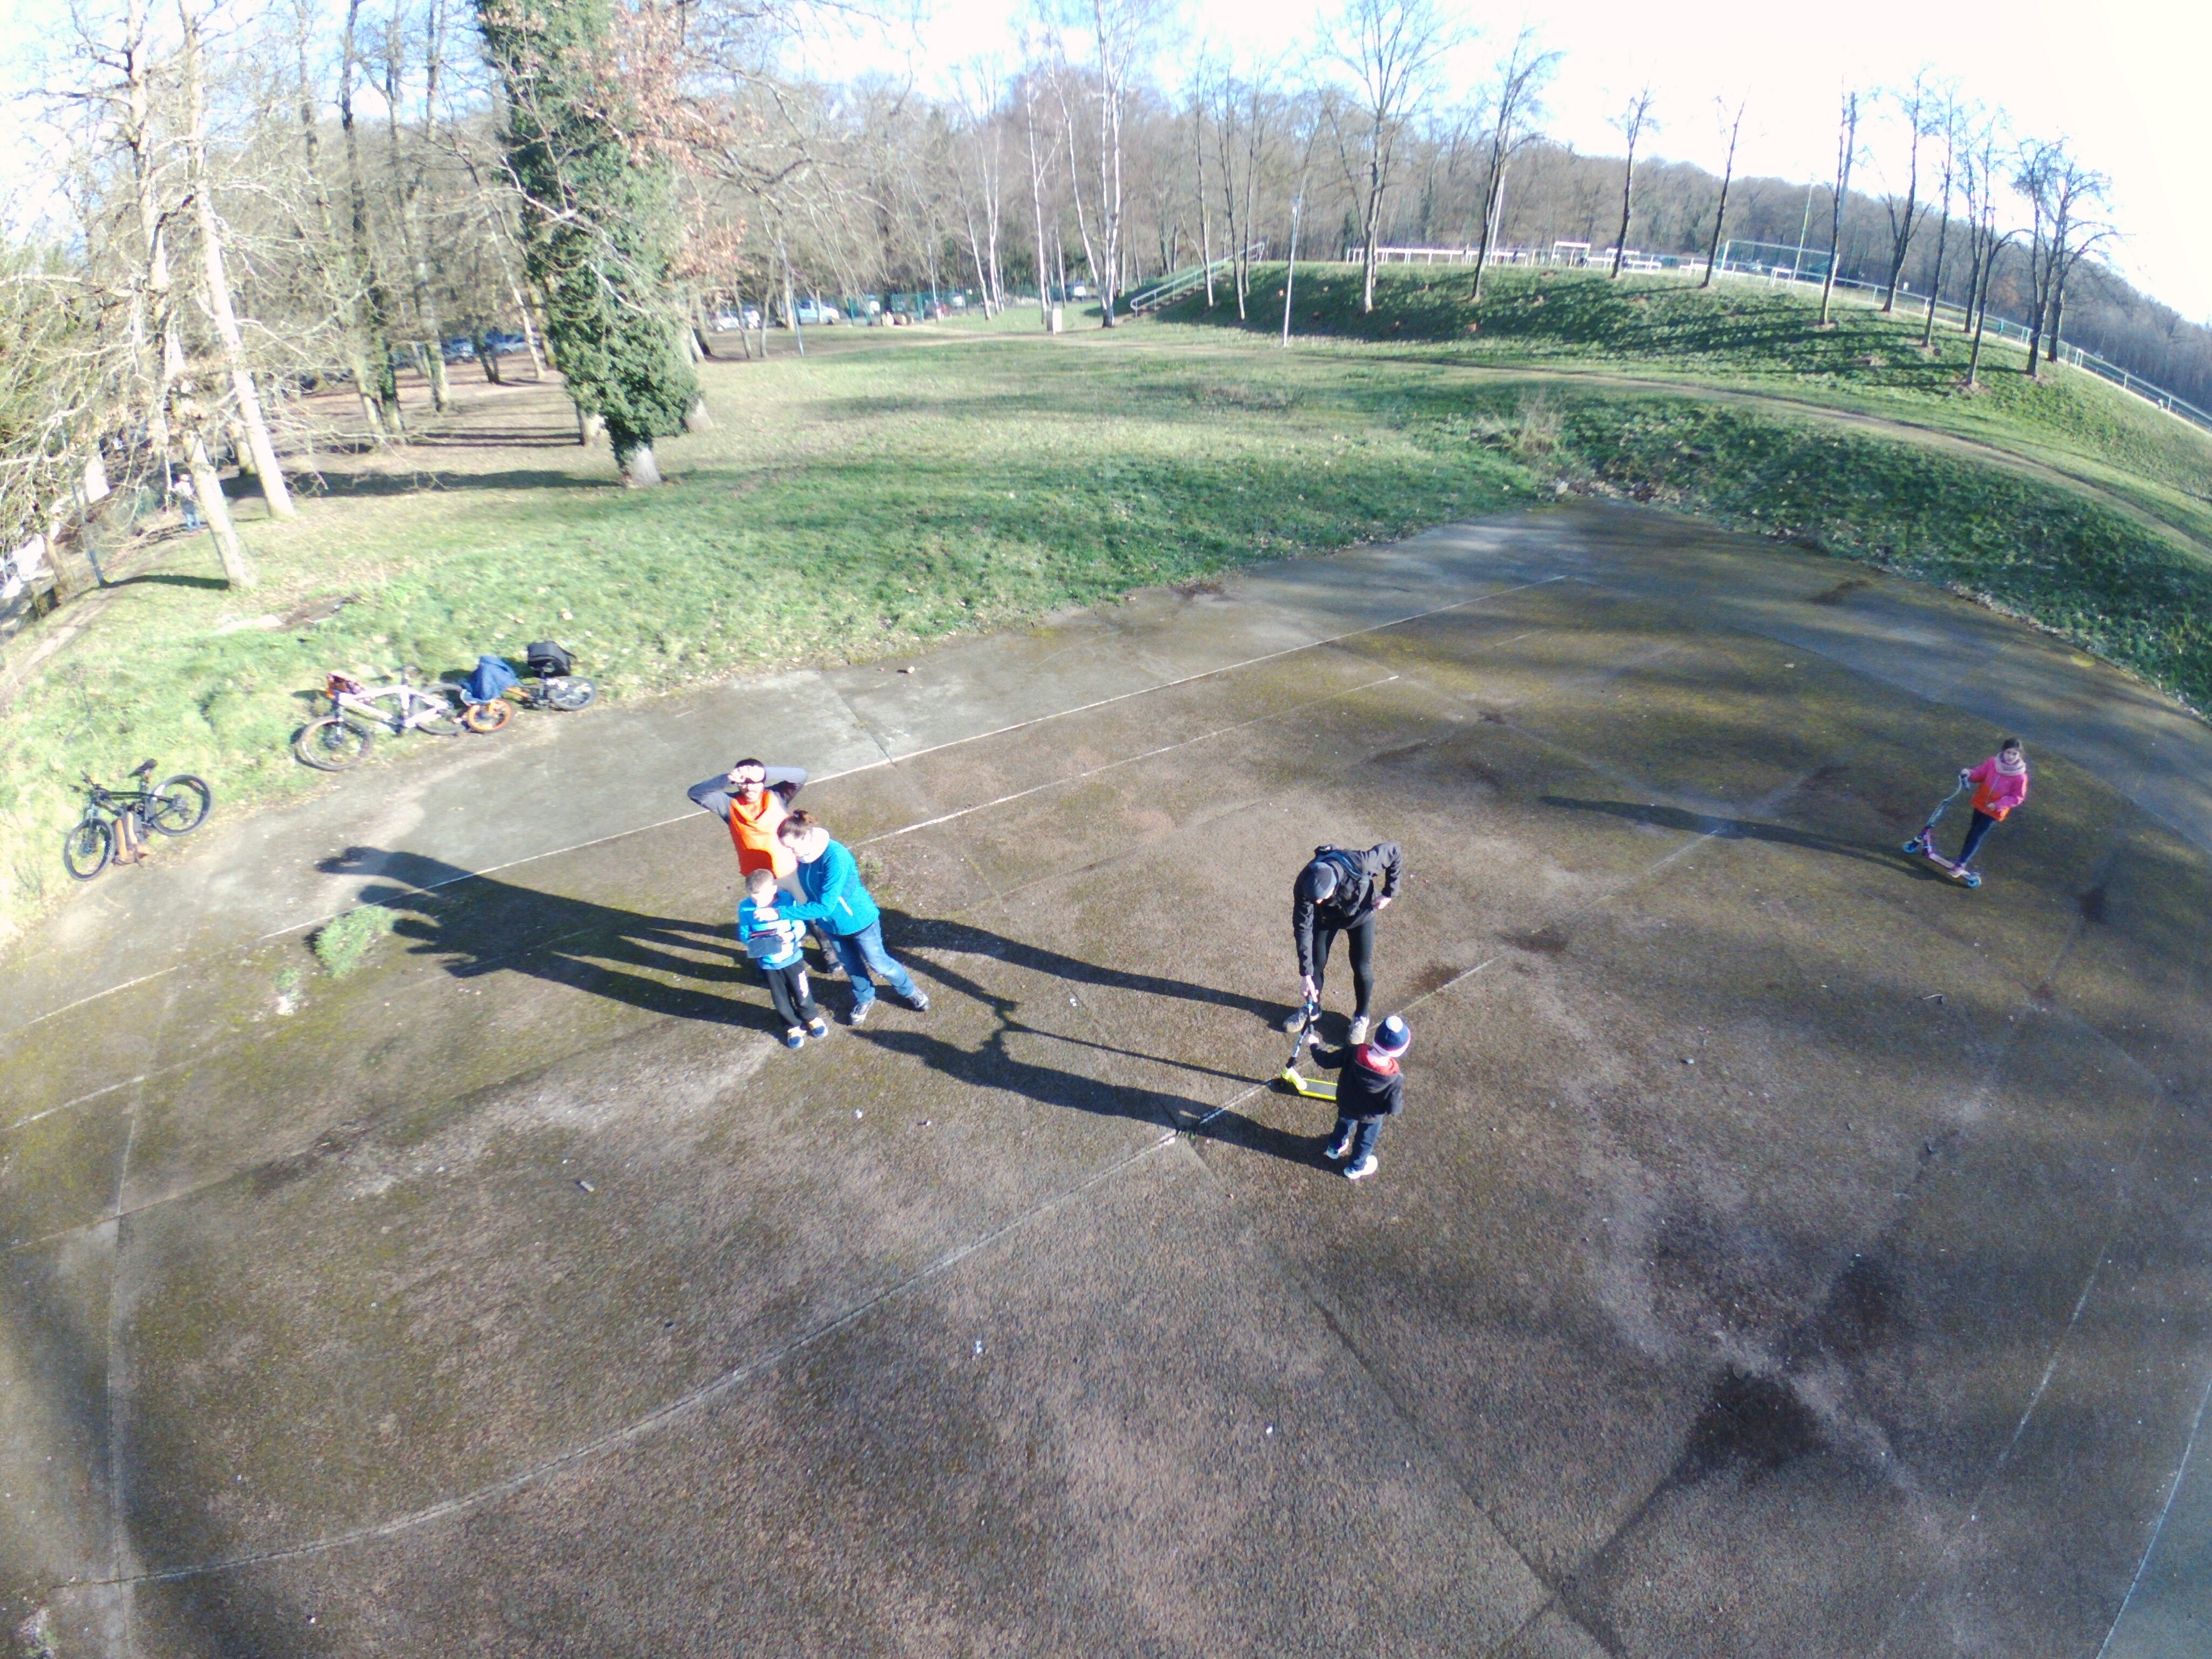
\includegraphics[width=\textwidth]{Bebop_A}}
        \caption{Precence of shadows}
    \end{subfigure}
        ~ %add desired spacing between images, e. g. ~, \quad, \qquad, \hfill etc. 
      %(or a blank line to force the subfigure onto a new line)
    \begin{subfigure}[b]{0.38\textwidth}
        \frame{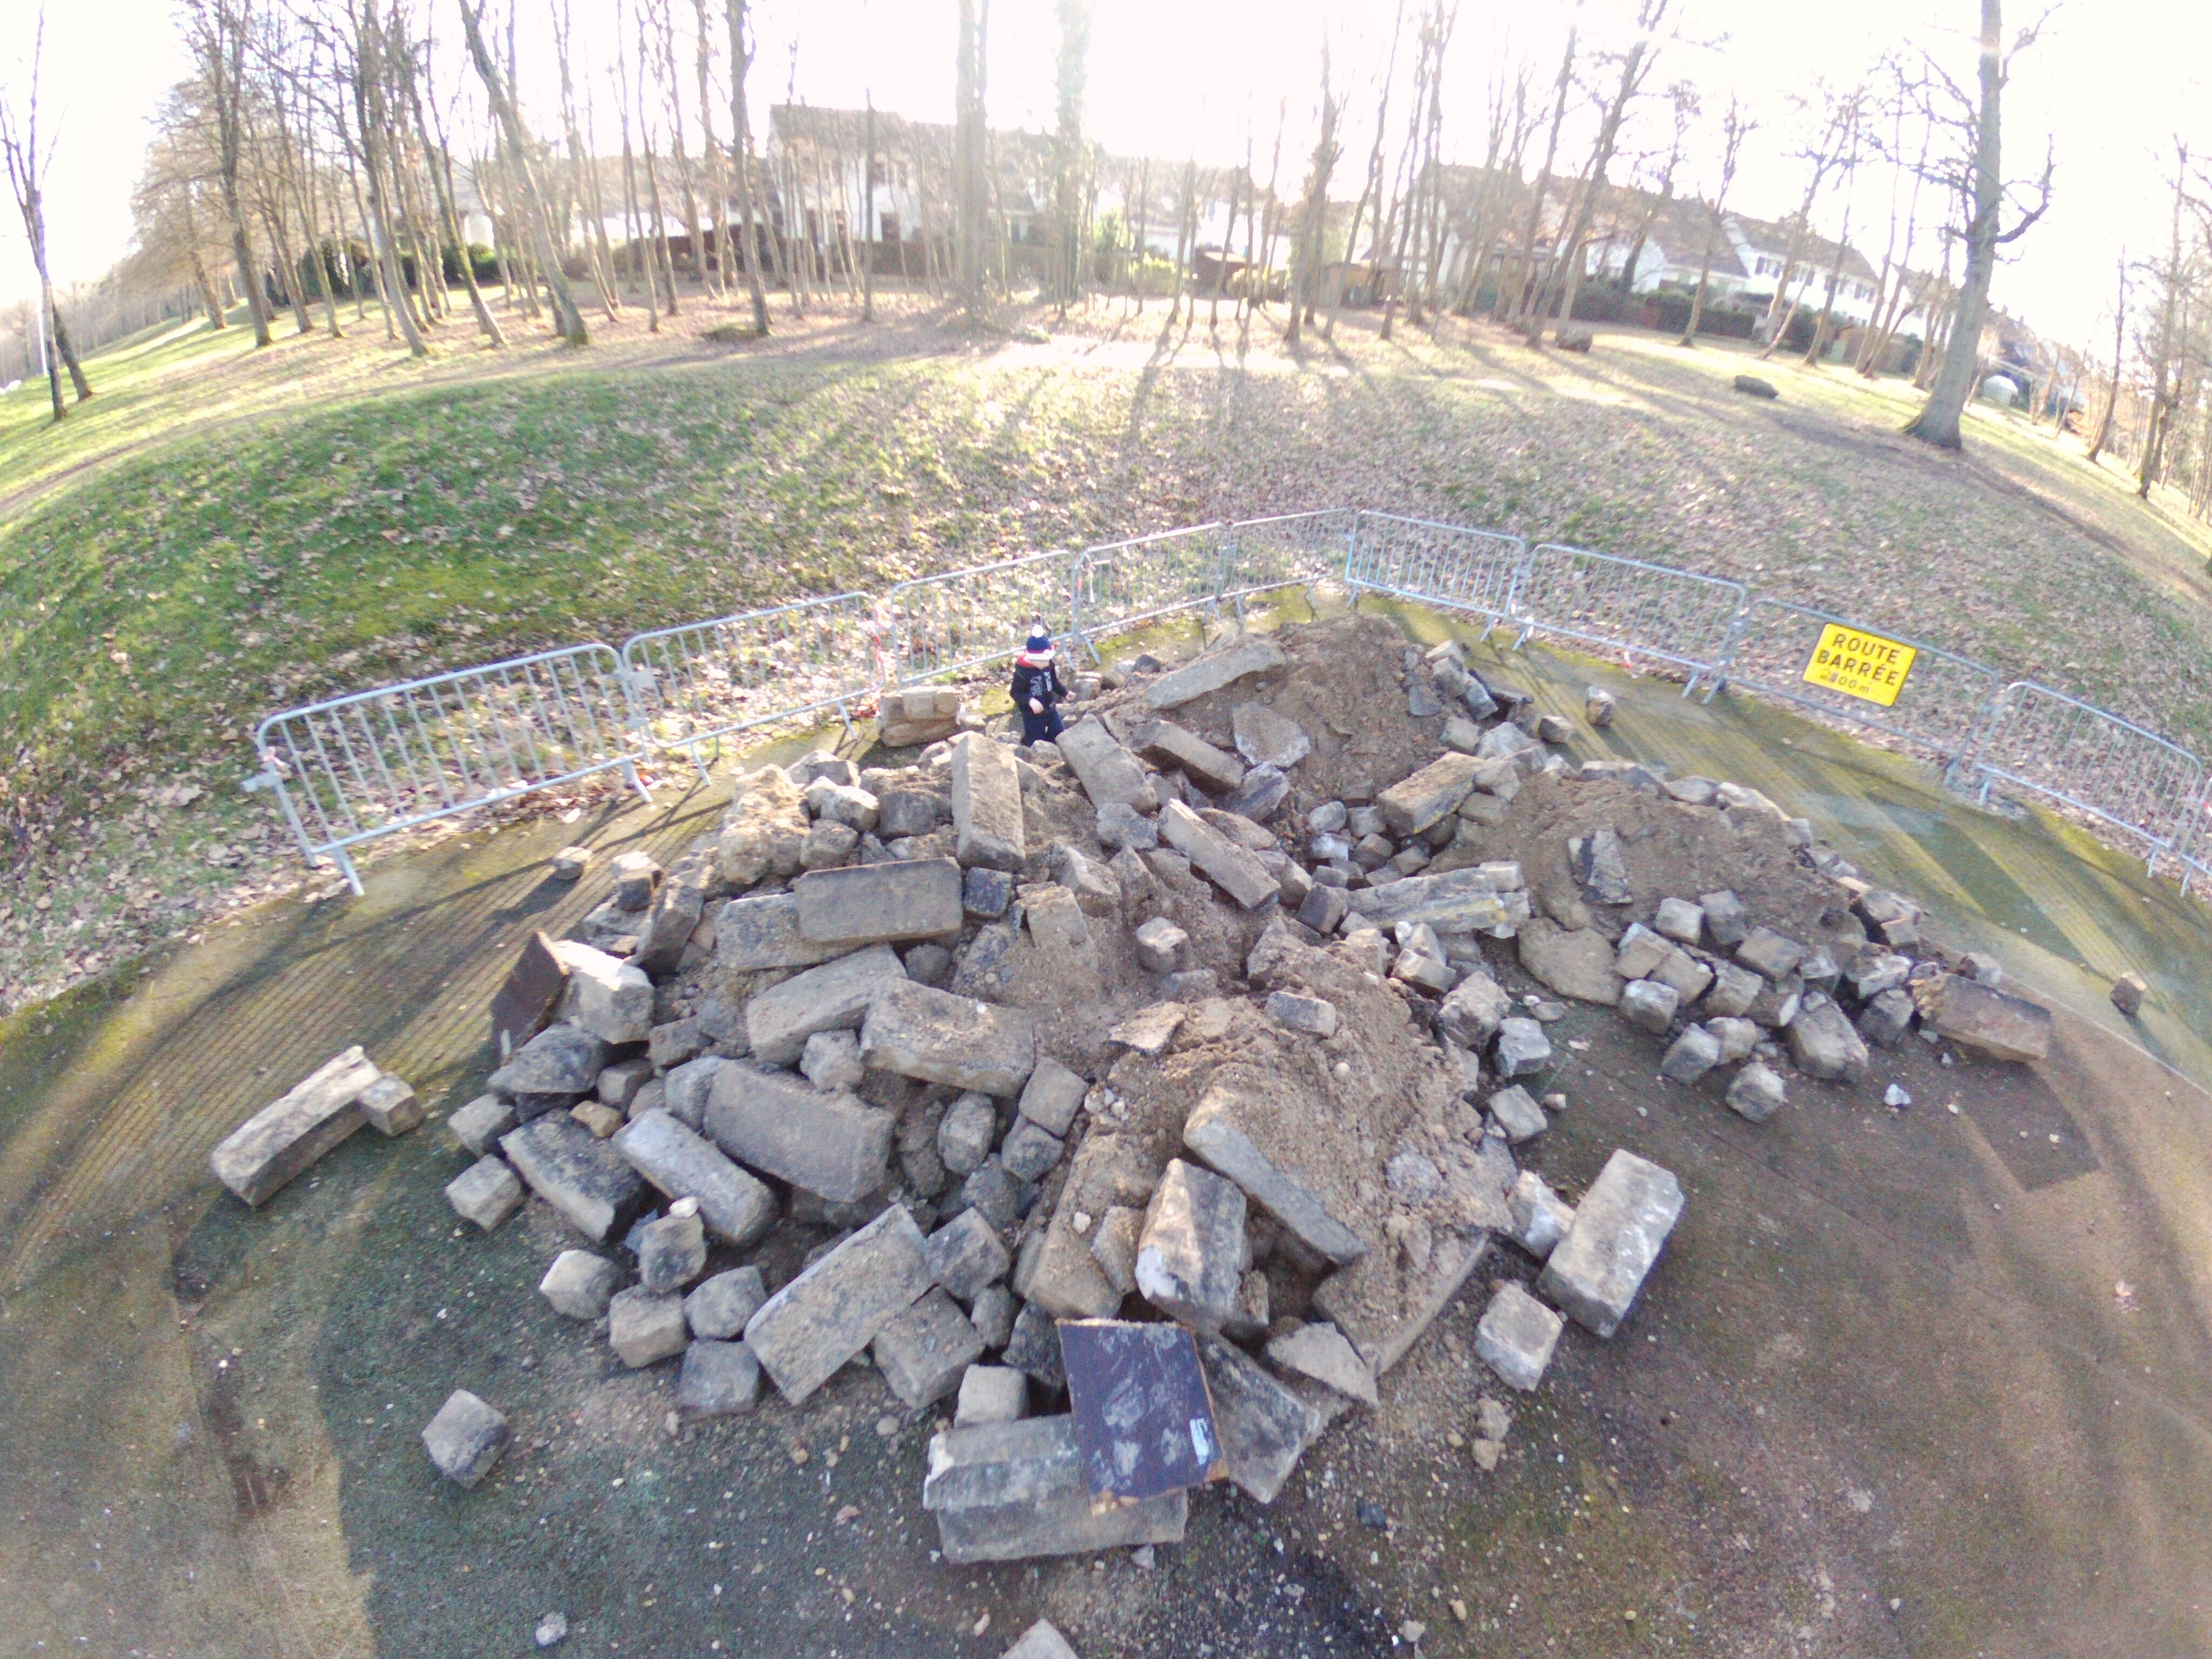
\includegraphics[width=\textwidth]{Bebop_B}}
        \caption{Saturations}
    \end{subfigure}
        ~ %add desired spacing between images, e. g. ~, \quad, \qquad, \hfill etc. 
      %(or a blank line to force the subfigure onto a new line)
    \begin{subfigure}[b]{0.38\textwidth}
        \frame{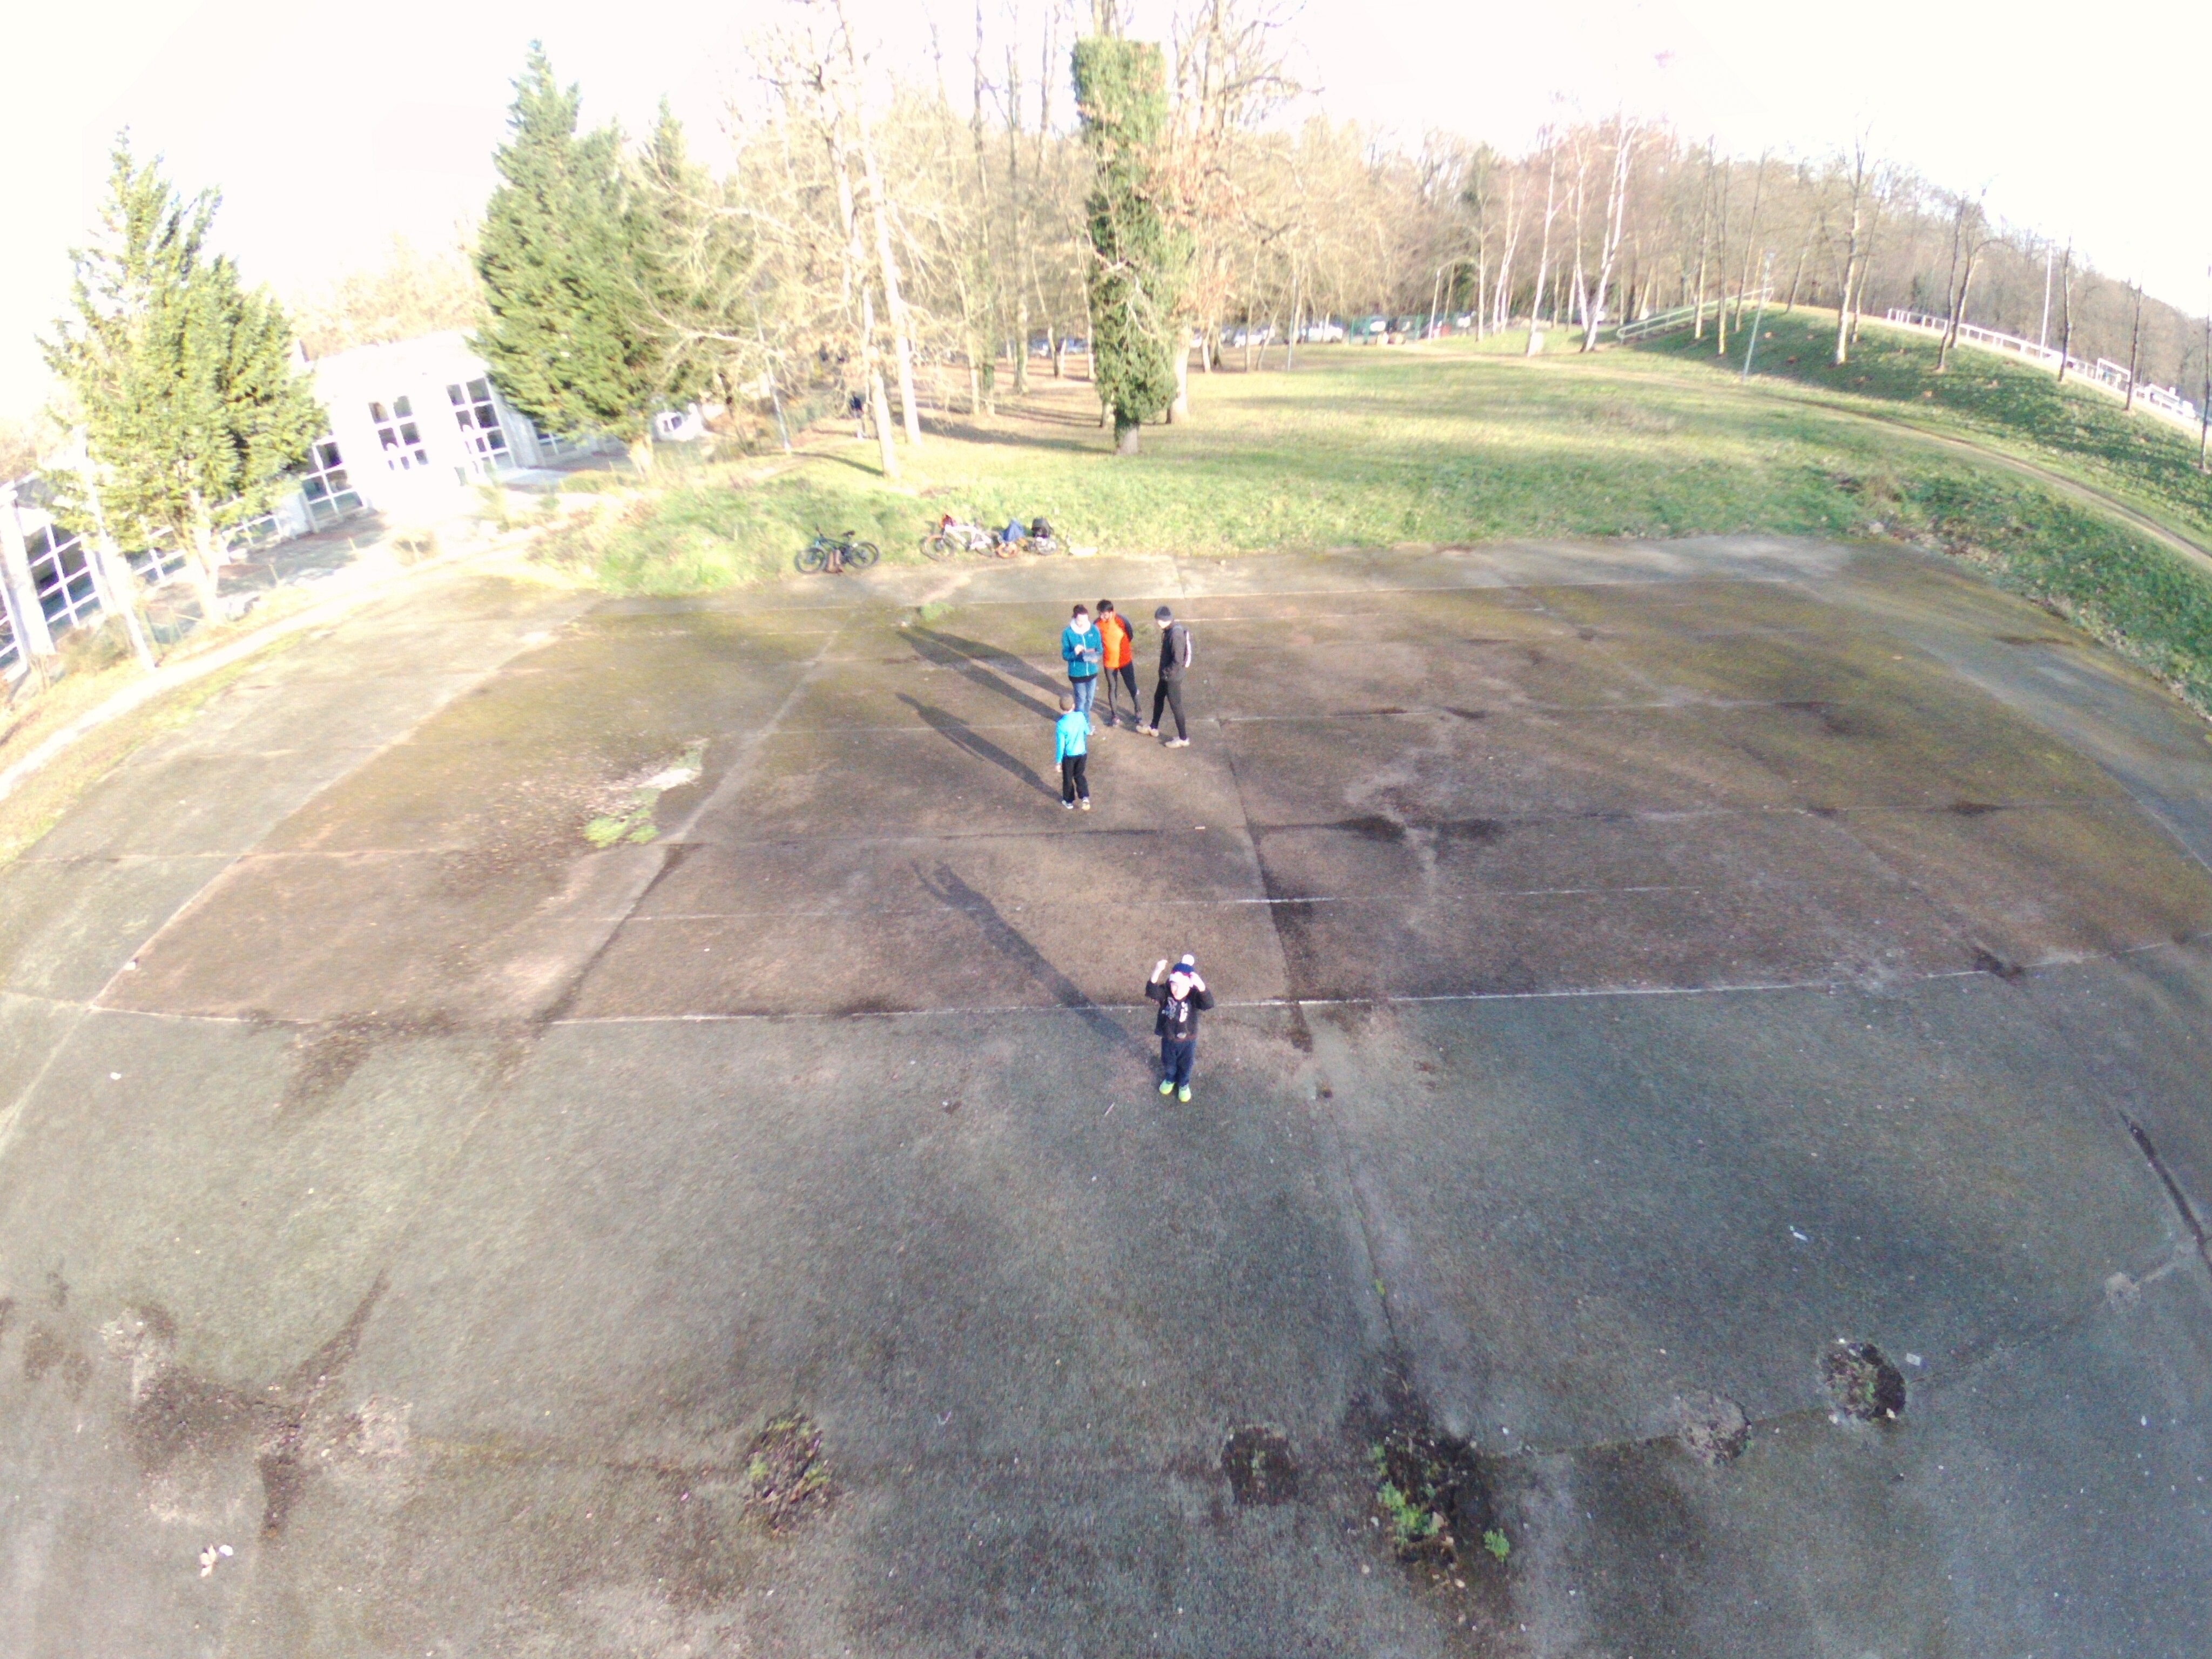
\includegraphics[width=\textwidth]{Bebop_C}}
        \caption{Change of scale}
    \end{subfigure} 
    \caption{Some examples of image degradations present in aerial imaging and UAV applications.}\label{fig:img_drone_degradations}
\end{figure}

In addition to the problems related to the complex scene conditions, we must consider that a drone is subject to sudden changes in the environment, such as wind gusts, which can affect its stability and modify the visual information given by the on-board sensors. In such cases, the vision algorithms for drone navigation must process the input information fast enough to provide answers and transform them into real-time decision actions.

In the literature, we can find a large number of works that deal with drone navigation. Among these works, we can say that the different approaches are strongly related and motivated by the application's aim and the conditions in which it is carried out. However, we can differentiate two main vision-based techniques for UAV navigation; 1) localization and mapping and 2) obstacle avoidance.

Simultaneous Localization and Mapping (SLAM) falls within the first group techniques, where drone navigation is a consistent result. This technique estimates the drone's local pose and builds a 3-d model of its surroundings employing visual sensors.  The Visual Odometry (VO) \citep{Scaramuzza.Fraundorfer:RAM:2011} is responsible for the robot motion estimation while the maps are built with occupancy grid algorithms \citep{Thrun.Bu:AI:1996}. . According to the image information used to perform a SLAM, we can classify these approaches into feature-based methods, which extract a set of image features (e.g., lines, points) in a sequence of images, and direct-based methods, which make use of the image intensity information to estimate the structure and the motion of the robot.

The use of SLAM techniques for UAV navigation presents remarkable advantages. Feature-based methods can use various feature detectors, which typically count with an optimization stage to produce fast algorithms. Direct-based methods have the advantage of being robust to image degradations; they can lead better with images with texture and blurred zones; besides, the map produced is of an acceptable resolution. Interestingly, the strengths of the first group of methods are the weak points of the second and vice versa. A method that tries to gather the benefits of both approaches is the Semi-direct Visual Odometry \citep{Forster.Pizzoli.ea:ICRA:2014}; however, in general, the SLAM methods work in indoor environments, where the illumination conditions are static or controlled.

On the other hand, there are approaches for drone navigation that favor the avoidance of obstacles. This capability is essential for achieving free collision missions in both indoor and outdoor environments. A recurrent solution, as we early mentioned, is the multi-sensor data fusion. \cite{Gageik.Benz.ea:ACCESS:2015} present a platform using low-cost ultrasound and IR sensors; however, despite the obtained results, it utilizes several sensors to retrieve environment information, and yet, it does not get a perceptual representation of the scene due to the low resolution and perceptive capacity of the sensors. On the other hand, vision-based techniques for obstacle avoidance could identify obstacles and, in some cases, classify the found object \citep{Li.Ye.ea:IROS:2016}. 

We can classify the visual methods for avoidance of obstacles into two groups. The first, SLAM-based techniques, make use of the principles above. The 3-d reconstruction provides accurate and sophisticated maps and allows the air vehicle to travel with more information about the environment. In \citep{Moreno-Armendariz.Calvo:ICMEAE:2014}, takes this advantage to develop an obstacle avoidance approach for static and dynamic obstacles.

The second group is the flow-based methods which historically, were inspired by the navigation of insects such as bees \citep{Srinivasan.Gregory:PTBS:1992} or flies \citep{Franceschini.Ruffier.ea:InTech:2009}. Many insects in the wild identify obstacles through the intensity of light. During the flight, their eyes produce an optical flow that provides accurate spatial information. Currently, there are also works inspired by the behavior of the human eye \citep{Al-Kaff.Meng.ea:IVS:2016}. The technique measures the object size from the idea that objects in the robot's vision field are more significant as the obstacle is close.

The techniques for obstacle detection and avoidance present interesting characteristics and ideas. Notwithstanding, its implementation is strongly linked to an application under certain conditions. In consequence, Their use would involve a recalibration or readjustment of parameters. Given the conditions in which a drone can operate, it is necessary to have more general and non-supervised methods.

The most efficient algorithms to date are those based on Neural Network (NN) architectures and supervised learning techniques. Nevertheless, these techniques have remarkable disadvantages that question their usability and applicability in real-life drone missions. From a practical and even economic point of view, there is a limit to the number of applications in which we can use supervised methods given the fact that we need a lot of annotated data. The collection and the correct labeling of data representing a problem are valid only for a small number of applications.

The need for abundant information comes with high computational times required for model learning, ranging from a couple of hours to weeks. Of course, we can minimize this variable by increasing our machines' computing power; however, today, only those with large computing infrastructures can afford to train models with hundreds of billions of parameters.  

The above statement introduces the next disadvantage of deep neural network-based learning models: hyperparameters. We can roughly divide hyperparameters into two categories, 1) optimizer hyperparameters, which include learning rate, batch size, and the number of epochs and 2) model-specific hyperparameters, including the number of hidden layers, the first hidden layer, and the number of layers. Choosing the appropriate hyperparameters plays a crucial role in the success of neural network architectures because they control the learning algorithm's behavior, define the network structure and how the network is trained. Although there are methods to optimize their choice, generally, this task is a heuristic process, and their fine-tuning is a function of the specific application. It is possible to follow some rules based on experience, copy the same values from some other problem or make the setting by trial and error, though we cannot know the best value for a hyperparameter.

\subsection*{Scope of the Thesis}
The interaction between computer vision and applications made with unmanned aerial vehicles is extensive. This collaboration has generated new methodologies and approaches, both theoretical and practical, but has also given way to new research questions. So, we want to detail the scope and focus of this thesis work.

First of all, this thesis work is motivated mainly by my profile and interests in robotics and control theory, specifically in air vehicles. Knowing the fundamental limitations of aerial robots and the complexity of drones' applications, we explore computer vision theory to propose algorithms that improve and provide assistance in drone navigation tasks. In this sense, we are interested in studying the scene's perceptual information for their treatment and interpretation.

We focus primarily on the vision processing problems before the image object recognition: object detection and segmentation. We argue that scene understanding, through object recognition, is a key to UAV navigation, especially when the tasks are developed in complex, uncontrolled environments. From this perspective, we focus on using low-level image features to extract perceptual information. 


Throughout this work, we develop algorithms that use such primitives in conjunction with statistical and geometric tools from computer vision and signal theory. The developed algorithms provide solutions to the recognition and scene understanding problem's variants, such as the classification, identification, and detection of objects from a qualitative point of view, always looking for the application's physical meaning. Instead of using supervised methods, we focus on decomposing the image information from the point of view of signal theory and physics to use it later on non-supervised or mathematical morphology methods. So it is worth mentioning that the practical aspect linked to the implementation and the generation of solutions in real-time are not a priority.

Regarding the nature of the input data, we use only color or black and white images as input information, favoring monocular cameras among the wide range of visual sensors reviewed previously. This choice allows replicating the algorithms with low-cost cameras that can be easily embedded in a drone.

One last point about the focus of this work is about the type of computer vision techniques. The algorithms proposed in this thesis are based on traditional computer vision techniques, that is, non-deep learning techniques. This decision is consistent with drone applications' nature, where there are not necessarily rich enough annotated databases to apply the most sophisticated artificial intelligence models.

\section*{Objectives of the Thesis}\label{sec:objectives_of_the_thesis}

In this Ph.D. thesis, we aim to develop general computer vision algorithms considering the challenges and needs of UAV navigation. In this context, the primary objective is to propose a new methodological framework for decomposing images prior to detecting objects and understanding scenes. As we mentioned before, the idea is to apply this framework to assist in control and decision-making in drone navigation tasks. Therefore, the framework must be robust to image degradations existing in environments with uncontrolled conditions, in addition to being independent of the choice of specific parameters for its operation.

During the thesis, we consider many specific drone tasks, such as:

\begin{enumerate}[label=\roman*]
	\item \textbf{Recognition} is a classic computer vision problem responsible for determining whether an image contains an object, characteristic, or exercise. Some variants of this problem are the classification, identification, and detection of objects from which many specialized tasks emerge. For example, content-based image search, pose estimation, optical character recognition, reading of 2-d codes, facial recognition, shape recognition, among others.
	\item Environment awareness.
	\item Detection and avoidance of obstacles.
	\item Identification and following of targets.
\end{enumerate}
Given these tasks, the work focuses on the scene understanding problem. To deal with this problem, we deepen the study of low-level image primitives such as contours, color, texture, and texture color. Therefore, some secondary objectives involve building a representative feature space using concepts from signal theory, geometry, and statistics, in addition to concepts from human perception.

The idea is to gather these features under an unsupervised framework without specific parameters, using traditional machine learning and segmentation algorithms. Figure \ref{fig:general_diagram_framework} a general diagram of the framework we propose. The first stage of the framework consists of extracting the primitives from the image, here we work with contours, color, texture, and the relationship between color and texture. The second block of the framework exploits the perceptual information contained in the extracted primitives. Finally, the framework's third block applies different methods (supervised or unsupervised) to the image's feature space to solve various computer vision problems.  Although the framework itself is an ambitious goal, in this thesis, we present several algorithms that apply the framework methodology with one or more features to solve different computer vision problems such as object detection and recognition, image retrieval systems, perceptual object boundaries detection, and image segmentation.

The interest of obtaining a representative space of the image information from low-level hand-made features lies in the possibility of using it in a semi-supervised pipeline. By injecting annotated information into the frame, it might make generalizations and obtain medium- or high-level features such as the importance of color and texture information to a human when segmenting an image.

\begin{figure}[!ht]
    \centering
    \includegraphics[width=\textwidth]{general_framework_diagram}        
    \caption{Proposed framework for object detection and scene understanding.}\label{fig:general_diagram_framework}
\end{figure}

Several secondary objectives are present throughout the study of each of the low-level primitives and their resulting features.

\begin{itemize}
	\item \textbf{Framework implementation.} This objective refers to the first stage of implementation in simulated and off-board environments. In a second moment, to the implementation in a real platform. The latter requires the search for a portable platform capable of real-time operation.
 
	\item \textbf{Framework functional evaluation.} Comparison of the obtained results regarding the approaches of state of the art.
 
 	\item \textbf{Framework validation.} Real test deployment taking into account the constraints of portability and real-time on the industrial scale.
 
\end{itemize}

Finally, this thesis aims to show that traditional computer vision methods are (still) a reliable option to develop object detection and recognition for relatively complex tasks. Especially in the current context of computer vision, where there are hundreds of algorithms based on neural networks and artificial intelligence for image segmentation and object detection that are highly performant but lack a physical (and in many cases logical and argued) interpretation of its results. Furthermore, these algorithms are in trouble when it comes to image analysis of complex scenarios or applications where there is no database rich enough to do the learning process.


\section*{Organization of the Document}
We explore three low-level primitives during this thesis; contours, color, and texture. The organization of this document follows, to some extent, the evolution of the construction of the vision-based framework for object detection and aid in drone navigation. This thesis will then be decomposed into two parts:

\begin{enumerate}
	\item A part dedicated to studying the contours of the image, in which we review in detail some of the classic methods for obtaining image contours. We use this information in conjunction with the \textit{a contrario} method and the Gestalt organizing laws to detect and identify landing targets.
	\item The second part main topic is the study of the properties of color and texture of an image. In the first moment, we are interested in the global distribution of this information and the existing metrics to measure the similarity between the distributions; we apply and validate these concepts in a retrieval image system. Subsequently, we extend the study of color and texture in images, exploding the local distribution of these primitives and studying the influence of color information on the generation of textures in an image. We propose a completely unsupervised framework for the detection of perceptual boundaries. Furthermore, we explore different strategies to obtain the segmentation of natural images using the obtained perceptual boundaries.
\end{enumerate}

More specifically, the chapters contained in the three sections are structured as follows:

\begin{itemize}
	\item \textbf{Chapter \ref{ch:landing_target_detection}} addresses the bases of the Gestalt theory, including the grouping laws and the Helmholtz principle. We formalize these concepts of human perception mathematically and formulate a non-parametric algorithm that follows an unsupervised framework based on an image's contours. We use the developed framework in the autonomous drone landing problem, specifically detecting and identifying landing targets.  The chapter also presents a review and a quantitative comparison of different traditional methods for extracting image contours.
	
	\item \textbf{Chapter \ref{ch:color_texure_representations}} presents a detailed review of the different ways to represent the color and texture information in an image. The chapter contains a review of various color spaces and their main properties and an introduction to the different techniques for characterizing textures in the literature. Such information is of relevant importance in the construction of the framework and the approaches to measure similarity between distributions.
	
	\item \textbf{Chapter \ref{ch:similarity_measures}} presents the analysis between different similarity measures between distributions, showing the advantages and disadvantages of each of them. In particular, we focus on the theory of optimal transport through the Earth Mover's Distance. We show the advantages of this metric over traditional similarity measures using an image retrieval system based on an image's global color and texture information.
	
	\item \textbf{Chapter \ref{ch:spectral_image_decomposition}} delves into the physical and human perception aspects of Gabor's filters. We show the steps involved in designing an optimized and efficient Gabor family of filters. The proposed filter family models and captures the texture information through an energy-efficient decomposition of the image. Such spectral decomposition of the image deals with Heisenberg's uncertainty principle. The chapter presents the description of parameters that allow complete customization of the filter family according to the application.
	
	\item \textbf{Chapter \ref{ch:complex_spectral_image_decomposition}} brings an analysis of the texture information present in color images, showing the strong relationship between those two features. Using the spectral analysis of an image with the previously defined Gabor filters, we generate a feature space that simultaneously captures the color and texture information. We show the richness of such feature space by performing unsupervised image segmentation only using simple clustering techniques.
	
	\item \textbf{Chapter \ref{ch:perceptual_object_boundaries_detection}} introduces a framework for the detection of perceptual boundaries of objects present in natural images. This framework brings together concepts addressed in this document, such as the spectral decomposition of images, the optimal transport as a true metric, and the relationship between color and texture information. Besides, using the hierarchical segmentation technique, we segment natural images in an unsupervised manner. We perform a quantitative and qualitative validation of our method using a known database.
	
	\item \textbf{Chapter \ref{ch:general_conclusion}} contains the general conclusions of the thesis and addresses the different possible research lines as a continuation of this work.
	
\end{itemize}